%!TEX root = ..\MainFile.tex
\chapter{ПЕРВАЯ ГЛАВА} % (fold)
\label{cha:chapter_name}
В следующем пункте надо описать на каких системах ставились эксперименты, что изучалось больше всего и привести какие-нибудь графики.
С другой стороны, наверно, можно сначала описать модель Вичека, а потом под нее подбирать какие-то результаты. Хотя у вичека не так.
Еще надо аккуратно повыписывать, конспективно, к каждой статье о чем там речь (ну типа физика, или какие конкретные животные.) \cite{_handling_????}
%!TEX root = ..\MainFile.tex
\section{Групповые явления в жизни животных} % (fold)
\label{sec:AnimalFlocking}
\epigraph{Если сто бегунов как один бегут,\\
Это можно назвать так и сяк.\\
У лошадей это будет табун,\\
У рыб это будет косяк.}{Машина Времени}
	\subsection{Методы наблюдения и сбора информации} % (fold)
	\label{sub:ExperimentalMethods}
	Главной сложностью в выполнении экспериментального наблюдения за группой животных или, тем более, насекомых, заключается в трудности отслеживания траекторий отдельных особей. Это связано с тем что рассматриваемые колонии или группы
	\begin{itemize}
		\item  состоят из множества индивидов, которые
		\item выглядят очень похоже
		\item и в основном очень быстро перемещаются
	\end{itemize}
	Кроме того, необходимо учитывать крайнее разнообразие живых организмов, за перемещением которых необходимо наблюдать, поскольку, как уже говорилось во введении, изменение поведения при обьединении в группы наблюдается для широкого разнообразия типоразмеров животных - начиная от бактерий в пробирке \cite{csahok1997,keller1971} и заканчивая китами на океанских просторах \cite{makris2009}.
	Несмотря на совсем неочевидные методы решения этих проблем, изучению стадного поведения (flocking bechavior) на протяжении многих лет посвящалось значительное внимание. Можно заметить что особенно остро (хоть и не в такой формулировке) этот вопрос стоял в 20-е годы XIX столетия на территории Одеской области, которая подвергалась массовым нашествиям саранчи, однако без компьютерного оборудования или без достижения теории ренормализационных групп достичь каких-либо результатов было невозможно.

	Итак, возвращаясь к теме этого пункта, вкратце рассмотрим использующиеся сейчас методы регистрации траекторий индивидов в стаде (стае). Условно, их можно разделить на две неравные группы: в одну отнесем так или иначе методы с использованием визуальных средства (т.е. фото- и видео-камер, в комбинации с различного рода маячками или метками), а в другую сравнительно недавно начавшие применяться методы с использованием GPS-систем. И если применение методов из второй групы не вызывает никаких технических вопросов (кроме, очевидно, закрепления такого рода устройств на исследуемых индивидах), то на методах первой группы следует остановиться подробней.

	Классическим может считаться метод измерение скорости по изображениям частиц \cite{raffel2007}. Обычно он применяется для измерения скорости потока жидкости или газа: в исследуемую среду вводится краситель, состоящий из броуновских частиц, и наблюдая за перемещением этого вещества становится возможным определять линии тока в исследуемой среде. Применимо к самодвижущимся частицам метод успешно был применен Czir\'{o}k и соавторами\cite{csahok1997}, которые при помощи фазово-контрастной микроскопии исследовали групповое движение молекул.

	Когда речь заходит об исследовании стай птиц (стад животных), размер индивидов больше, однако в отличие от бактерий область перемещения слабо ограничена. Тогда движение записывается напрямую на камеру, с тем чтобы в дальнейшем восстановить отдельные траектории. К примеру, в 70-х годах аерофотосьемка использовалась для определения расположения отдельных индивидов во время сбивания африканских буйволов в стадо \cite{sinclair1977}. Однако использования одной камеры для фиксирования перемещений группы рыб или птиц явно недостаточно, поскольку как-то необходимо учитывать расстояние от камеры до особи. Чтобы обойти эту сложность, например, Бекко и соавторы \cite{becco2006} огриничили движение рыб по высоте используя плоский и широкий аквариум.

	Использование нескольких камер для сьемки стай с разных точек в дальнейшем требовало трудоемкой обработки результатов для получения трехмерной картины. Получение стереографических изображений с последующей обработкой позволило определить расстояния между соседними индивидуумами в стаях скворцов и чернозобиков \cite{major1978}. В менее давних исследованиях был обработан метод преобразования фотографий стаи в трехмерные коспьютерные модели, что позволило получить мгновенные снимки положения сотен скворцов в стае \cite{ballerini2008}, однако в задаче восстановление траекторий движения все еще остается поле для исследования.

	По мере развития технологий, стало возможным создать маячки GPS, достаточно маленькие, чтобы их можно было закрепить на животном или птице не мешая ему. К сожалению, с увеличением количества отслеживаемых индивидов возрастает и стоимость исследования. С другой стороны, такого рода устройства обладают ограниченной точностью в определении местоположения. Несмотря на приведенные выше ограничения, были проведены исследования пар \cite{biro2006,nagy2010}, или даже шестерок \cite{dellariccia2008} тренированных голубей.

	Помимо вышесказанного, в настоящее время увеличение точности сонаров и разработка определенной технологии применения, в которой океан выступает в роли акустического волновода позволило использовать их для единовременного наблюдения за огромными количествами рыб на больших территориях океанического шельфа. \cite{makris2006}

	Подводя итоги, можно отметить увеличение роли комьютера в накоплении и обработке экспериментальных данных. Текущая динамика позволяет надеяться что со временем будут получены данные не меньшей точности, чем получаемые во время численных экспериментов по различным моделям.
	% subsection subsection_name (end)

	\subsection{Основные результаты наблюдений} % (fold)
	\label{sub:ExperimentalResults}
	Поскольку экспериментальное наблюдение стадных явлений не является темой данной работы, мы не будем останавливаться подробно результатах полевых или лабораторных исследованиях, тем более что всестороннее освещение этого вопроса дано в работе Вичека~\cite{vicsek2012}. Однако для лучшего понимания распространенности в природе стадных явлений будет приведен краткий обзор наиболее характерных, с нашей точки зрения, работ, сгруппированных по исследуемому материалу. Итак, в разные годы обьектами исследования становились:
	\begin{enumerate}
		\item Внутриклеточные соединения \cite{chowdhury2006,keller1971}
		\item Колонии бактерий \cite{czirok1998,csahok1997}
		\item Насекомые \cite{buhl2006}
		\item Птицы \cite{ballerini2008,selous1931,dellariccia2008,biro2006,major1978,nagy2010}
		\item Рыбы \cite{cambui2012,makris2009,parrish1997}
		\item Млекопитающие, к примеру буйволы \cite{sinclair1977}
	\end{enumerate}
	Особняком в этом ряду стоят наблюдения за океаническим планктоном \cite{seuront2004}, и превышающие по своей численности наблюдения за любым другим типом обьектов наблюдения за поведением групп людей, например \cite{parisi2009,moussaid2011}.%ссылка про транспортные потоки

	Кроме того, в совершенно отдельную группу необходимо выделить лабораторные эксперименты, проводимые с неживыми обьектами - нематической жидкостью, колеблющимися металлическими стержнями, нано частицами в жидкости, микро роботами и тому подобным. \cite{schaller2010,turgut2008,blair2003}

	Теперь, приведем основные результаты, полученные в ходе наблюдений. Для начала, наобходимо четко разделять работы в которых исследования велись на плоскости (все кроме указанных далее), и в которых наблюдения велись в трехмерном пространстве \cite{cullen1965,ballerini2008,major1978,makris2009}. Хотя, как выяснилось, для рыб такое разделение не вполне необходимо. Но обо всем по порядку.

	Главный вывод, который в общем-то и не нуждается в подтверждении - это то, что существует отдельный класс перемещений группы индивидов как целого, и при этом перемещения отдельных индивидов оказываются упорядочены. То есть, при определенных условиях (чаще всего рассматривается различная плотность на единицу площади, или обеспеченность ресурсами в широком смысле слова) происходит спонтанное нарушение симметрии, и хаотическое движение сменяется упорядоченным. Как уже говорилось, это наблюдается на всех масштабах природы, и более того - совершенно не обязательно при этом прямое (визуальное или тактильное) взаимодействие между особями, и бывает достаточно опосредствованного взаимодействия через среду обитания \cite[с. 119]{vicsek2012}. %добавить информацию про молекулы, перекидывающие взаимодействие через жидкость в которой они живут
	Следующее наблюдение на которое указывают многие авторы - при нарушении симметрии возникает и дальний порядок связи, к примеру, рыбы могут изменять общее направление движения практически мгновенно \cite{cambui2012}, а птицы так-же быстро принимать решения о посадке. \cite{lukeman2010,major1978}.

	Но более того, самым удивительным явлется то, что у всех живых существ и неживых предметов, при движении которых проявляются стадные явления, качественный характер этих явления практически одинаков. %(Не считая сугубо трехмерных формаций, которые образуются в стаях птиц, однако и там можно выделить правильный ``параметр порядка'').
	\begin{figure}
        \centering
        \begin{subfigure}{.4\columnwidth}
                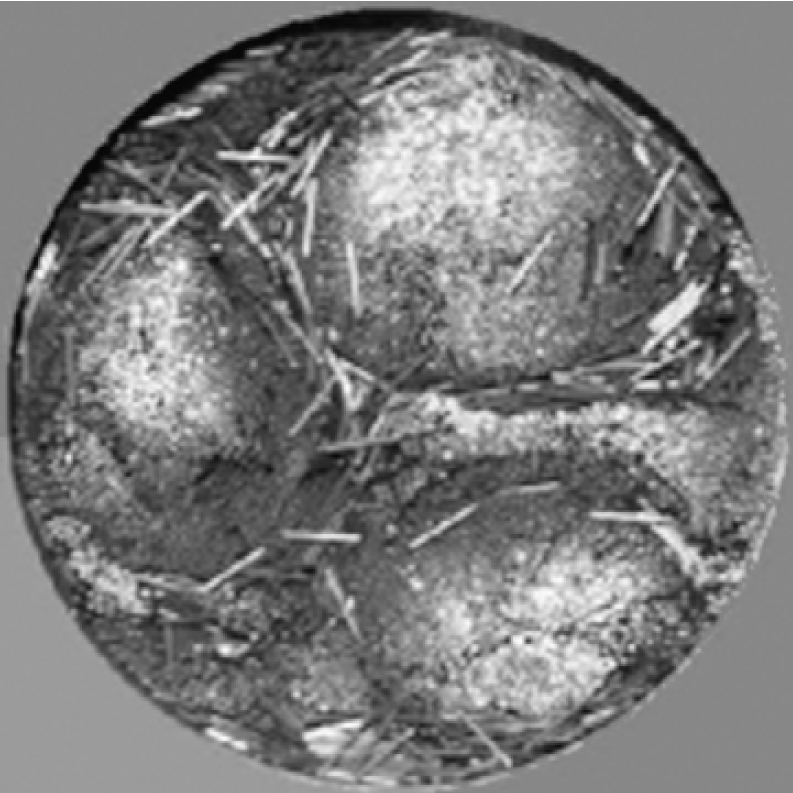
\includegraphics[width=\columnwidth]{Fig4_CollectiveMotion}
                \caption{A nematics}
                \label{fig:CollMot:nematics}
        \end{subfigure}%
        ~ %add desired spacing between images, e. g. ~, \quad, \qquad, \hfill etc.
          %(or a blank line to force the subfigure onto a new line)
        \begin{subfigure}{.4\columnwidth}
                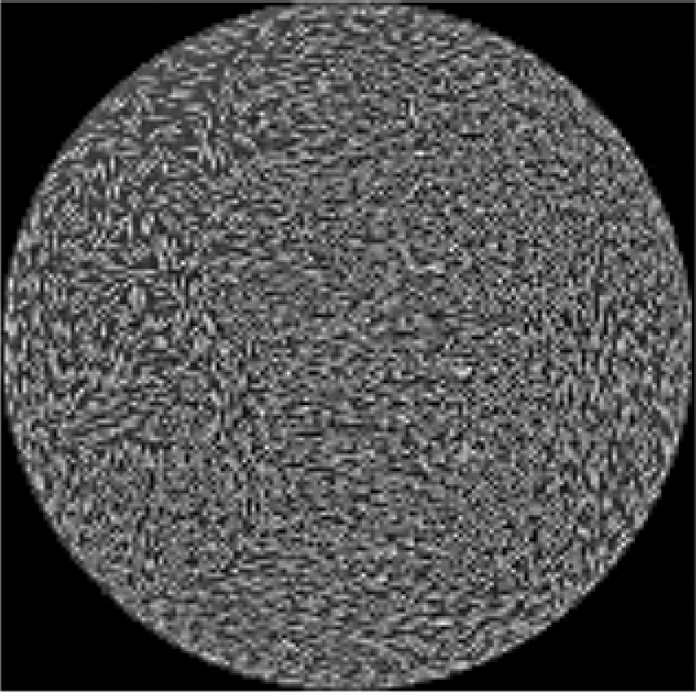
\includegraphics[width=\columnwidth]{Fig6_CollectiveMotion}
                \caption{A rods on wibe}
                \label{fig:CollMot:rods}
        \end{subfigure}
        \caption{Упорядочивание неживых обьектов}
        \label{fig:CollMot:NonLiving}
    \end{figure}
        ~ %add desired spacing between images, e. g. ~, \quad, \qquad, \hfill etc.
          %(or a blank line to force the subfigure onto a new line)
    \begin{figure}
    	\centering
        \begin{subfigure}{0.3\textwidth}
                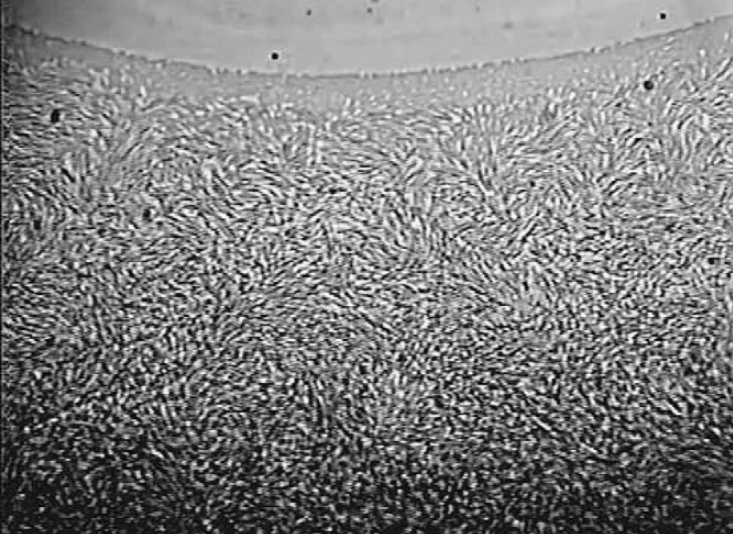
\includegraphics[width=\textwidth]{Fig11_CollectiveMotion}
                \caption{A bacteria 1}
                \label{fig:CollMot:bacteria}
        \end{subfigure}
        \begin{subfigure}{0.5\textwidth}
                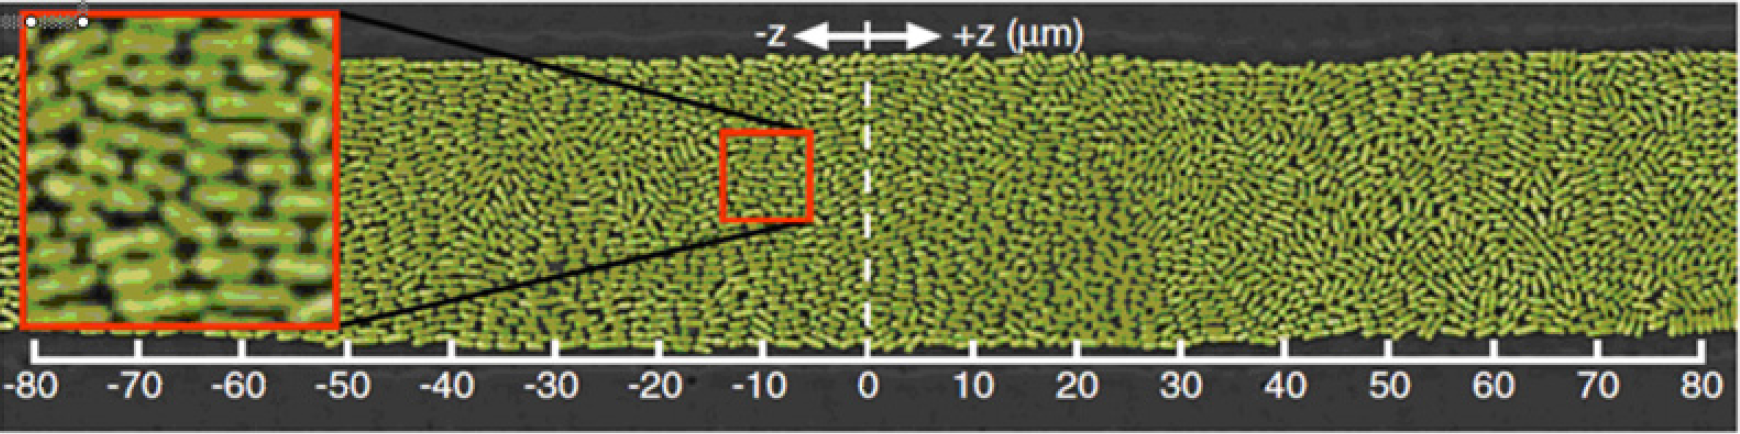
\includegraphics[width=\textwidth]{Fig15_CollectiveMotion_part}
                \caption{A moleculae}
                \label{fig:CollMot:moleculae}
        \end{subfigure}
        \caption{Микроскопические проявления групповой динамики}
        \label{fig:CollMot:microscpoic}
    \end{figure}
    \begin{figure}
    	\centering
        \begin{subfigure}{0.4\textwidth}
                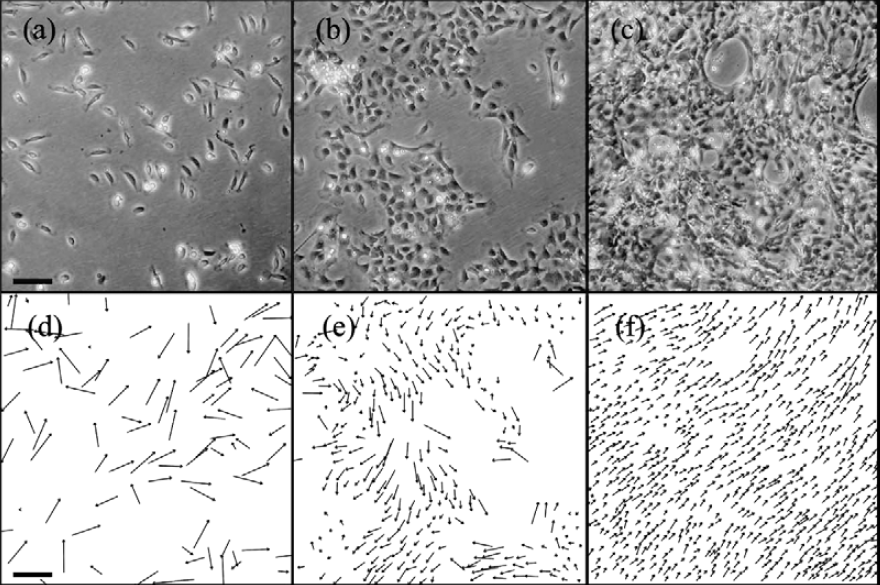
\includegraphics[width=\textwidth]{Fig17_CollectiveMotion}
                \caption{A fishes}
                \label{fig:CollMot:fishes}
        \end{subfigure}
        \begin{subfigure}{0.4\textwidth}
                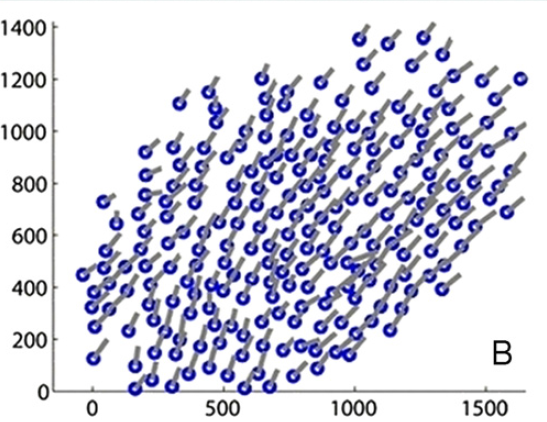
\includegraphics[width=\textwidth]{Fig29_CollectiveMotion_part}
                \caption{A ducks}
                \label{fig:CollMot:ducks}
        \end{subfigure}
        \caption{Макроскопические проявления группового движения}\label{fig:CollMot:macroscopic}
	\end{figure}

	Наглядно это можно рассмотреть на рис. \ref{fig:CollMot:NonLiving}, \ref{fig:CollMot:microscpoic}, \ref{fig:CollMot:macroscopic}. Особенностью всех представленных на изображениях обьединений является то, что они расположены на плоскости. И как мы видим, возникает два типа упорядоченностей, иногда (как на рис. \ref{fig:CollMot:nematics}) проявляющихся единовременно: это упорядоченное движение в спонтанно выбранном направлении, или упорядоченное обращение вокруг некоторого центра. Видно также, что для совершенно, казалось бы, различных обьектов групповое поведение является очень схожим.

	Что же касается перемещений, не ограниченных в двух плоскостях, то нам хотелось бы заострить внимание на трех моментах. 

	Во-первых, в обьемном пространстве также наблюдаются все вышеперечисленные упорядоченные перемещения: птицы сбиваются в стаю и летят в выбранном направлении \cite{dellariccia2008}, насекомые кружат вокруг улья \cite{buhl2006} и т.п.

	\begin{wrapfigure}{r}{0.5\textwidth}
	  \vspace{-20pt}
	  \begin{center}
	    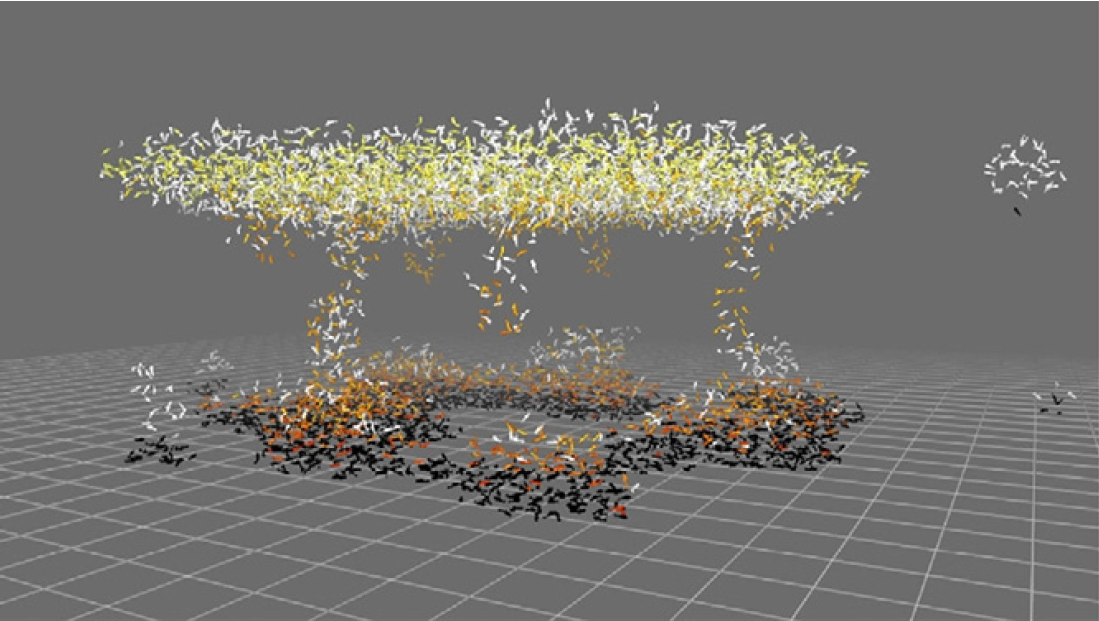
\includegraphics[width=0.48\textwidth]{Fig57_CollectiveMotion}
	  \end{center}
	  \vspace{-20pt}
	  \caption{Расслоение косяка рыб}
	  \label{fig:FishSplitting}
	  \vspace{-10pt}
	\end{wrapfigure}

	Во-вторых, и это является особенностью косяков рыб, возможно расслоение трехмерной группы на более плоские подгруппы, с наличием соединяющих (цилиндрических) столбов. Предполагается, что это это связано с ``мотивацией'', например, молодая стерлядь во время нереста предпочитает подниматься выше, а более старая опускается вниз. \cite{axelsen2000} При этом наблюдаются структуры как изображенные на рис. \ref{fig:FishSplitting}

             \begin{figure}
    	\centering
                \begin{subfigure}{0.4\textwidth}
                    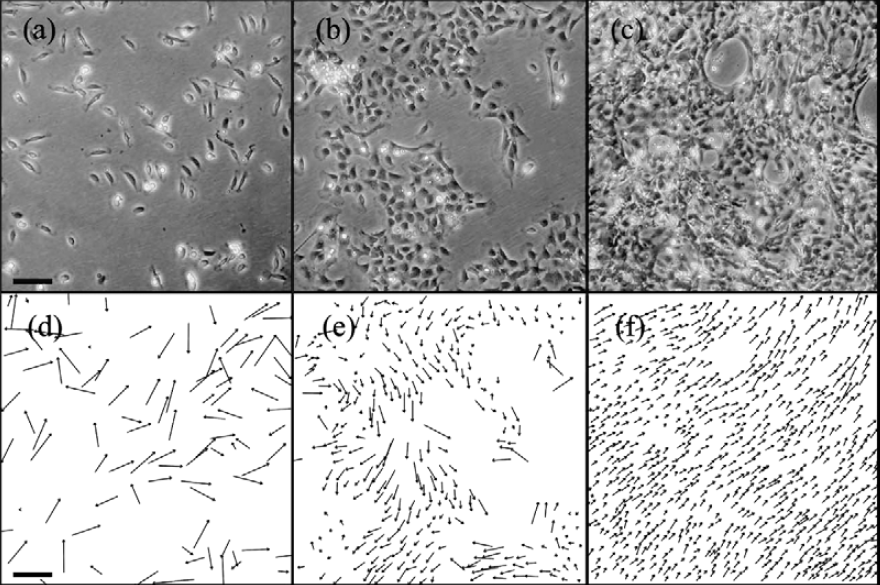
\includegraphics[width=\textwidth]{Fig17_CollectiveMotion}
                    \caption{A fishes}
                    \label{fig:CollMot:Birds}
                \end{subfigure}
                \begin{subfigure}{0.4\textwidth}
                    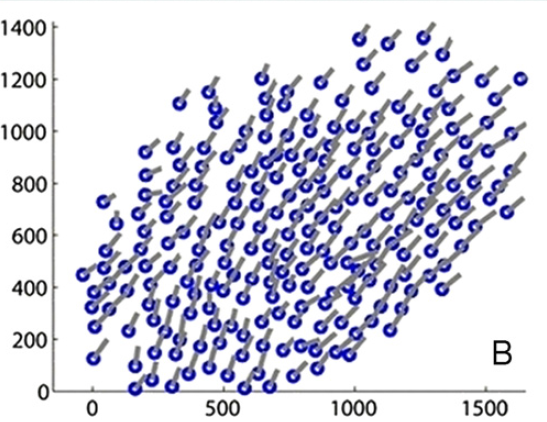
\includegraphics[width=\textwidth]{Fig29_CollectiveMotion_part}
                    \caption{A ducks}
                    \label{fig:CollMot:Plancton}
                \end{subfigure}
                \caption{Макроскопические проявления группового движения []}\label{fig:CollMot:Volumetric}
	\end{figure}

	И в третьих, поскольку основное внимание при наблюдениях в трехмерном пространстве уделялось птицам и рыбам, групповая динамика которых хоть и обладает большим количеством подобных черт, все-же разнятся в том что стаи птиц не расслаиваются по высоте, тем более ярко проявляется аналогия между пространственными формированиями птиц и морского планктона []
    \marginpar{необходимо уточнить что имелось ввиду в \cite{seuront2004}}%уточнить!!!!
	
            \textcolor{red}{В дальнейшем в этой части можно указать что в групповых явлениях наблюдаются ``лидеры'', которые могут задавать движение. Еще где-то надо сказать что фазовый переход переходит или при уменьшении шума, или при увеличении плотности, наверно в следующем пункте}

            % subsection основные_результаты_наблюдений_за_системами_демонстрирующими_группувую_динамику (end)

            \subsection{Количественные характеристики группового движения} % (fold)
            \label{sub:NumCharCollMot}
                Не смотря на то, что подобность движений различных типов обьектов очевидна, для какого-либо исследования нельзя обойтись без количественных характеристик явления.
                Укажем отдельно характеристики обьектов, которые участвуют в коллективном движении:
                \begin{enumerate}
                    \item все они похожи друг на друга
                    \item они перемещаются с почти постоянной скоростью и способны изменять направление движения
                    \item они взимодействуют находясь на эффективном расстоянии, и посредством этого изменяют направление движения в стремясь к выравниванию
                    \item направление движения подвержено шуму определенной амплитуды
                \end{enumerate}

            Рассматривая же обьекты в совокупности необходимо заметить что при определенных условиях происходит (скачкообразный) переход от разупорядоченного к упорядоченному движению. Такое явление называется фазовым переходом. Наиболее знакомые всем нам фазы, в которых может пребывать фещество - газообразная, жидкая и твердая, переходят одна в другую при изменении как минимум одного внешнего параметра - температуры. При этом плотность выступает в роли {\itпараметра порядка} - некоторой величины, которая однозначно характеризует фазу вещества.

            Пользуясь этой аналогией, и помня о том что изменяется только направление движения каждого обьекта, в качестве параметра порядка было естественно определить следующей величиной:
            \begin{equation}\label{eq:OrederParam}
                \varphi = 1/{N v_0} |{\sum\limits_{i=1}^n \vec{v_i}}|
            \end{equation}
            Параметром порядка, согласно этому определению, является модуль средней скорости, нормированной на единицу. В уравнении \ref{eq:OrederParam} $N$ - полное число обьектов, $v_0$ - средний модуль скорости обьектов в системе. Понятно, что если движение неупорядочено, то скорости обьектов направлены случайным образом, и такая сумма будет стремиться к нулую. Если же скорости направлены вдоль некоторого выбранного направления, то параметр порядка стремится к единице. Разумеется как и всяческий статичтический параметр, выражаемый через средние величины, это выражение имеет смысл только при больших $N$, иначе величина флуктуаций из-за кадого обьекта будет слишком высокой.

            Из статистической физики нам известно, что фазовый переход может происходить как в равновесной (замкнутой), так и в неравновесной системе. Ввиду того что в групповом движении, согласно рассматриваемой модели, участвуют самодвижущиеся частицы становится понятно что системы с групповой динамикой сугубо неравновесны. Неравновесная статистическая физика в последнее десятилетие выделилась в отдельное направление физики, со своим словарем, обьектом исследований и характерными процессами, вызывающими наибольший интерес исследователей в текущий момент времени. И потому, возможно, было бы предпочтительнее модифицировать модель или провести аналогии с фазовыми переходами, рассматриваемыми в рамках равновесной статистической физики. \cite{vicsek2012}

            Эта идея, однако, кажется не приемлимой по нескольким соображениям: Во-первых, в системах, демонстрирующих групповую динамику, наблюдаются совершенно не характерные для равновесной термодинамики явления, такие как ``пробки'' или флуктуации гигантского числа частиц []. А во-вторых, статистическая механика имеет дело с количеством частиц стремящимся к бесконечности ($10^23$), и в рамках этого допущения определяет остальные понятия, в то время как явления группового перемещения наблюдаются при числе частиц редко превышающем десятки тысяч.

            Интересным было замечание [], указывающее на значительную аналогию в поведении систем, демонстрирующих групповую динамику, и феромагнитных систем. К примеру, рассматривая критические экспоненты, связанные с параметром порядяка вида:
            \begin{equation}
                \sigma \sim |1-\eta/\eta_c|^-\gamma
            \end{equation}
            позволяют вычислить критические индексы $\gamma$. При этом получается, что критические индексы вычисленные, скажем, по модели Изинга, и вычисленные из (численных) экспериментов с системами, демонстрирующими групповую динамику оказываются в хорошем согласии между собой. За более полной информацией о параллелях между феромагнетиками и системами с групповой динамикой смотри []\marginpar{doi:10.1088/0305-4470/30/5/009}.

            Итак, резюмируя, в системах с коллективными эффектами происходит фазовый переход, при этом параметром порядка выступает средняя векторная скорость \ref{eq:OrederParam}, а в качестве ``температуры'' - шум, т.е. некоторое добавочное воздействие, которое случайным образом изменяет направление движения каждого обьекта в рассматриваемой системе. Возникает вопрос - единственный ли это параметр, который может повлиять на фазу системы и привести к фазовому переходу? Как было экспериментально проверено Камбуи \cite{cambui2012} и многими другими, фазовый переход в системе взаимодействующих обьектов также возможен при увеличении плотности. Кроме ``обычного'' фазового перехода, при котором изменяется только направление скорости обьектов, иногда наблюдается явление в котором, при увеличении плотности, уменьшается скорость перемещения обьектов, и образуется ``пробка''[] \marginpar{Keller-segel, \cite{keller1971}}
            % subsection NumCharCollMot (end)
            На этом мы заканчиваем, сложность систем требует вдумчивого и основательного подхода, и потому изначально было предложено значительное количество компьютерных моделей \cite{reynolds1987,vicsek1995,gregoire2004,nagy2007,schubring2013}, и лишь потом, на основании результатов, полученных в численных экспериментах, были разработаны теоретические подходы к групповому движению. \cite{tu2000,kulinskii2005,bertin2006,ratushnaya2007,vicsek2007,chepizhko2013,kulinskii2014}

% section групповые_явления_в_жизни_животных (end)
В главе про компьютеры основной упор на дискретные модели (собсно, Вичек, Грегуар, и тому подобные.) Обратить внимание на то, что они в основном используют вычислительные кластеры, и сослаться на их литературу.
Вообще, надо свести в одно место все ссылки, избавиться от взаимных ссылок, и выбрать самое интересное.
%!TEX root = ..\MainFile.tex
\section{Компьютерные модели групповой динамики} % (fold)
\label{sec:ComputerModelsOfHords}

\epigraph{Позабыты~хлопоты,~остановлен~бег~- \\
Вкалывают роботы, а не человек.}{Ю. Энтин - ``Вкалывают роботы''}
Как было сказано в разделе \ref{sec:AnimalFlocking}, основной сложностью в исследовании процессов, происходящих в рое, является невозможность уследить сразу за всеми представителями. В первую очередь проблема заключается в высокой технической сложности гарантированно отличить одну особь от другой.

    \subsection{Основные модели} % (fold)
    \label{sub:CompModelsBasics}
    Моделированием групповых эффектов начали заниматься в 70е годы несколько групп ученых - биологов, физиков и специалистов по компьютерной графике. 
    \begin{figure}
        \centering
        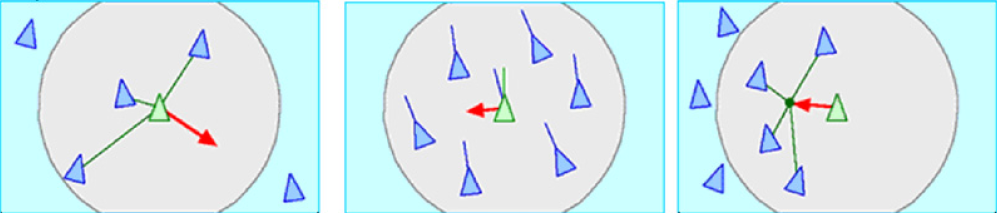
\includegraphics[width=\textwidth]{Images/Fig31_CollectiveMotion}
        \caption{Поведение, основное для модели Рейнольдса. (а) Разделение, с тем чтобы избежать чрезмерного скапливания боидов. (б) Выравнивание: боиды поворачивают в направлении средней скорости окружающих боидов. (в) Когезия: боиды смещаюстся в направлении центра масс окружения}
        \label{fig:ReynoldsModel}
    \end{figure}
    Первая широко известная модель была предложена Рейнольдсом~\cite{reynolds1987}. В его модели поведение обьектов (боидов) определялось из рассчета наилучшего визуального представления. Боиды могли демонстрировать три типа взаимодействия: избегание столкновений, следование в направлении ближайших боидов и стремление к центру масс стаи, рис. \ref{fig:ReynoldsModel}. С тем, чтобы привнести в изучение групповых эффектов количественный подход, была предложена модель, широко известная сейчас как ``модель Вичека''~\cite{vicsek1995}. Поведение частиц в этой модели определяется следующими соотношениями:
    \begin{equation}
        \vec{v}_i(t+1) = v_0 \frac{{\langle \vec{v}_i(t) \rangle}_R}{|{\langle \vec{v_j}(t) \rangle}_R|} + perturbation
    \end{equation}
    \begin{equation}
        \vec{x}_i(t+1) = \vec{x}_i(t)+\vec{v}_i(t+1)
    \end{equation}
    Здесь ${\langle \dots \rangle}_R$ обозначают усреднение (или суммирование) по всем частицам в радиусе $R$ вокруг $i$-й. Тогда $ \frac{{\langle \vec{v}_i(t) \rangle}_R}{|{\langle \vec{v_j}(t) \rangle}_R|}$ предоставляет нам единичный вектор в направлении средней скорости группы частиц. Такое выравнивающее правило не принимает во внимание характер взаимодействия, и потому модель может соответствовать когезии, взякости и тому подобному. Введение шума в модель может выполняться различными способами. В оригинальной работе было предложено следующее: поскольку единичный вектор однозначно соответствует углу, задающему направление, и скорость частиц также можно задавать в виде модуля скорости и единичного вектора направления, то тогда угол направления движения в момент времени $(t+1)$ получается следующим образом:
    \begin{equation}
        \vartheta_i (t+1) = \vartheta_i(t) + \Delta_i(t)
    \end{equation}
    где $\vartheta_i(t) = \arctan [{\frac{{\langle \vec{v}_i(t) \rangle}_R}{|{\langle \vec{v_j}(t) \rangle}_R|}}]$, и шум представлен $\Delta_i(t)$ - случайное число равновероятно выбранное из $[-\eta \pi,\eta \pi]$. Единственными параметрами модели является плотность $\rho$, модуль скорости частиц $v_0$ и уровень шума, определяемый $\eta < 1$. Параметром порядка становится 
    $\varphi = 1/{N v_0} |{\sum\limits_{i=1}^n \vec{v_i}}|$, как определно в уравнени \ref{eq:OrederParam}.

    Несмотря на кажущуюся простоту этой модели, она демонстрирует богатый спектр свойств, характерных для систем, демонстрирующих групповую динамику. В первую очередь это, конечно же, фазовый переход к упорядоченному движению. Помимо этого, варьируя указанные выше параметры модели, удавалось получить различные паттерны, характерные для групповой динамики, а именно вращающиеся ``цепи'', ``ленты'', ``мельницы'', ``марширующие группы'' и другие. При определенных условия возможно получение интересных результатов по таким вопросам как ГЧФ или формирование лент.

    Интересным вопросом является род фазового перехода. В своей оригинальной работе Вичек и соавторы показали, что наблюдается переход второго рода от разупорядоченного к упорядоченному движению. То есть, при переходе к термодинамическому пределу поведение параметра порядка недалеко от фазового перехода описывается
    \begin{equation}
        \varphi \sim [\eta_c(\rho)-\eta]^\beta
    \end{equation}
    \begin{equation}
        \varphi \sim [\rho-\rho_c(\eta)]^\delta
    \end{equation}
    Где [] и было получено что []
    Однако непрерывная природа фазового перехода была поставлена под вопрос Грегуаром и Шате~\cite{gregoire2004}, что привело к серии работ адрессующих этот фундаментальный вопрос коллективного движения. В результате экстенсивного исследования Шате и сооавторам~\cite{chate2008} удалось показать (численным экспериментом) существование т.н. переходного режима, в котором непрерывный характер перехода не зависит от модуля скорости частиц. \marginpar{Надо прочитать внимательно исходник}

    В то же время было обнаружено, что тип фазового перехода зависит от модуля скорости частиц и шума (вернее, того, как шум вводится в систему). Проведенные исследования показывают, что для малых скоростей $v_0 < 0.5$, даже в пределе скорости $v_0 \to 0$ наблюдается фазовый переход второго рода. Для больших скоростей фазовый переход аналогичен фазовому переходу первого рода. Косвенным свидетельством этого является формирование ``лент''.\cite{huepe2008}

    Существует две возможности привнести шум в систему: в виде случайного угла, на который поворачивается скорость частицы \textit{после} выравнивания с учетом направления движения окружения, и в виде случайного вектора, который добавляется ко всем частицам \textit{до} определения преимущественного направления движения. Первый вариант используется в модели Вичека, в то время как второй вариант был предложен Грегуаром и Шате~\cite{gregoire2004}. И как было показано численным експериментом~\cite{baglietto2008}, модель Вичека испытывает фазовый переход второго рода, в то время как при введении ``векторного'' шума возможно состояние при котором фазовый переход является переходом первого рода~\cite{aldana2009}.
    % subsection CompModelsCollMot (end)

    \subsection{Варианты модели самодвижущийся частиц} % (fold)
    \label{sub:VariantsOfVicsekModel}
    За годы прошедшие с момента создания модели Вичека, было предложено определенное количество моделей самодвижущихся частиц, воспроизводящих групповую динамику или отдельные характерные эффекты.~\cite{vicsek2012}
    Можно выделить два типа такого рода моделей - в одних прямо вводится правило выравнивания частиц, а в других рассматривается опосредственное взаимодействие, к примеру, через столкновения.
    % subsection VariantsOfVicsekModel (end)

    \subsection{Результаты численных исследований} % (fold)
    \label{sub:CompModelsResults}
    
    % subsection CompModelsResults (end)

% section section_name (end)

% chapter chapter_name (end)